% Chapter 1

\chapter{Introducción general} % Main chapter title

\label{Chapter1} % For referencing the chapter elsewhere, use \ref{Chapter1} 
\label{IntroGeneral}

En este capítulo se explica la importancia de la predicción de quiebra de empresas. Luego, se detalla el estado del arte actual respecto a esta temática. Se explican también las motivaciones detrás de este trabajo. Finalmente, se describen los objetivos y alcance del trabajo.

%----------------------------------------------------------------------------------------

% Define some commands to keep the formatting separated from the content 
\newcommand{\keyword}[1]{\textbf{#1}}
\newcommand{\tabhead}[1]{\textbf{#1}}
\newcommand{\code}[1]{\texttt{#1}}
\newcommand{\file}[1]{\texttt{\bfseries#1}}
\newcommand{\option}[1]{\texttt{\itshape#1}}
\newcommand{\grados}{$^{\circ}$}

%----------------------------------------------------------------------------------------

%\section{Introducción}

%----------------------------------------------------------------------------------------
\section{Predicción de quiebra de empresas}

Predecir si una empresa entra en quiebra es información de gran valor para distintos actores del mercado financiero. Acceder a esta información en tiempo y forma le permitirá a bancos, compañías aseguradoras, fondos de inversión o consultoras especializadas en riesgo crediticio tomar mejores decisiones en sus respectivas labores.

El presente trabajo es un emprendimiento personal orientado a la resolución de la problemática presentada. Para llevarlo a cabo, se utiliza el dataset de \textit{Taiwanese Bankruptcy Prediction}\citep{taiwanese_bankruptcy_prediction_572}, el cual contiene información financiera de empresas del mercado de Taiwán entre 1999 y 2009, y fue publicado por el \textit{Taiwan Economic Journal}\footnote{\url{https://www.tejwin.com/en/}}. Esta información será utilizada en el entorno de trabajo que se puede apreciar en la figura \ref{fig:diagBloques}. En este, se refina la información, se entrenan distintos modelos de machine learning, y se comparan dichos modelos a fin de elegir al mejor de ellos. Los resultados obtenidos se publican mediante un servicio web, para que los distintos interesados pueden consultarlos y utilizarlos según sus necesidades.

\begin{figure}[htbp]
	\centering
	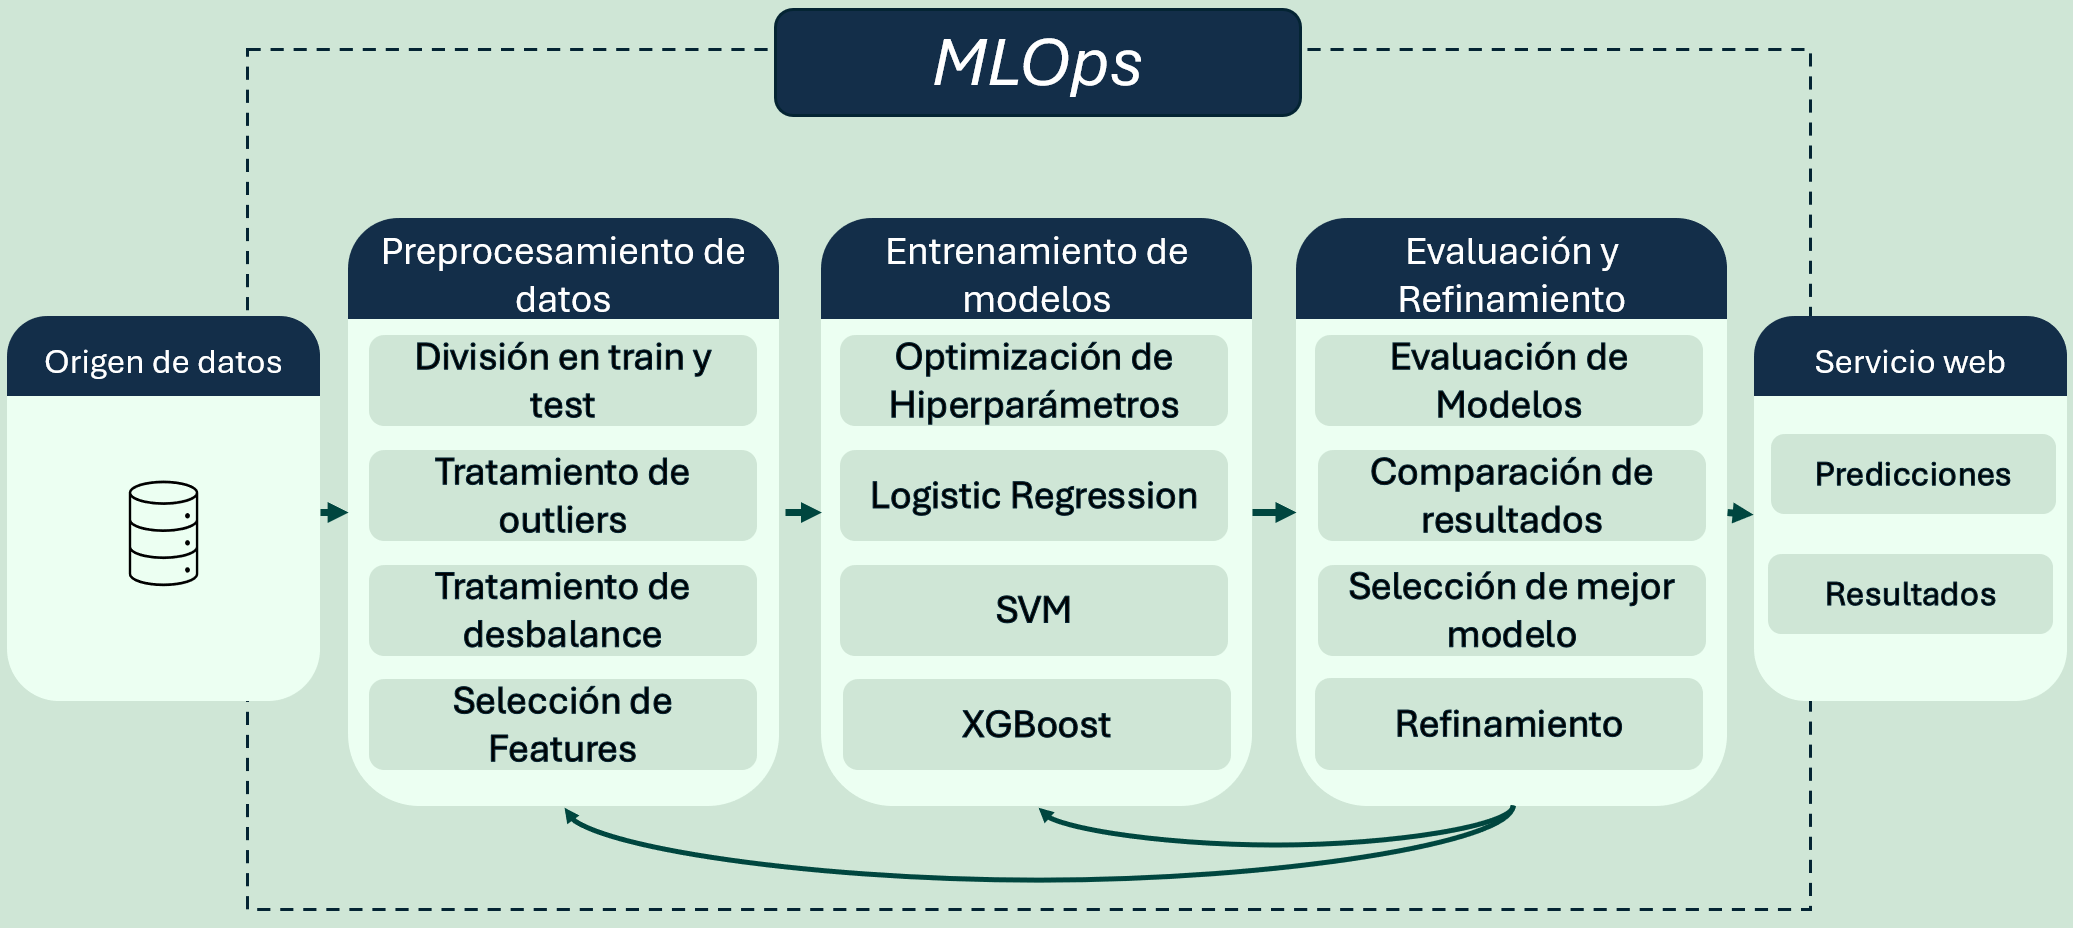
\includegraphics[width=\textwidth]{Figures/diagramaEnBloques.png}
	\caption{Diagrama en bloques.}
	\label{fig:diagBloques}
\end{figure}

%----------------------------------------------------------------------------------------

\section{Estado del arte}

Existen diversos estudios basados en el dataset de \textit{Taiwanese Bankruptcy Prediction}\citep{taiwanese_bankruptcy_prediction_572}. En algunos de ellos, como en \textit{Comprehensive Evaluation of Bankruptcy Prediction in Taiwanese Firms Using Multiple Machine Learning Models}, se exploran modelos de \textit{machine learning} tales como SVM (\textit{Support Vector Machine})\citep{model:svm} y \textit{Random Forest}\citep{model:rf}. En otros, se analiza cómo ciertas técnicas afectan a las predicciones finales. Por ejemplo, en \textit{Undersampling bankruptcy prediction: Taiwan bankruptcy data}\citep{10.1371/journal.pone.0254030} se estudian los resultados de aplicar técnicas de preprocesamiento de datos mediante \textit{undersampling}.

Independientemente de los modelos y de las técnicas de preprocesamiento utilizadas, los estudios actuales se limitan a presentar resultados numéricos y conclusiones sobre las herramientas utilizadas, pero ninguno permite utilizar los modelos obtenidos para realizar predicciones reales.

%----------------------------------------------------------------------------------------

\section{Motivación}

Este trabajo busca solucionar las siguientes problemáticas:

\begin{itemize}
\item Permitir a actores del mercado financiero predecir si una empresa entra en quiebra.
\item Resolver las limitaciones de trabajos actuales, en donde solo se presentan resultados numéricos y conclusiones.
\end{itemize}

Por ello, se diseña y desarrolla un sistema que implementa técnicas y modelos de \textit{machine learning}. Estos modelos, son entrenados, refinados y comparados para encontrar al que mejor prediga si una empresa entra en quiebra. Una vez seleccionado el mejor de ellos, se lo expone mediante un servicio web, a fin de que distintos interesados puedan utilizarlo según sus necesidades.

%----------------------------------------------------------------------------------------

\section{Objetivos y alcance}

Este trabajo busca crear y exponer, mediante servicio web, un sistema que prediga si una empresa entra en quiebra.
Para ello, se define un entorno de trabajo que se caracteriza por ser iterativo, reproducible y escalable, en donde se usa un dataset de origen público\citep{taiwanese_bankruptcy_prediction_572}. Sobre este dataset se aplicarán técnicas de preprocesamiento de datos para mejorarlo. Luego, se entrenarán modelos de \textit{machine learning}, que permitan realizar las predicciones deseadas. Estos modelos serán evaluados y comparados entre sí, a fin de encontrar al "mejor" de ellos. El mejor modelo y los resultados obtenidos serán expuestos mediante un servicio web, para que cualquier interesado pueda hacer uso de ellos. Sobre estos resultados se vuelven a aplicar las técnicas ya mencionadas, para poder refinarlos y reevaluarlos.

A partir de esto, se define el siguiente alcance:

\begin{itemize}
\item Análisis exploratorio de datos: se estudia al dataset en cuestión, para poder conocer mejor sus características, distribuciones, y potenciales errores a corregir.
\item Preprocesamiento de datos: se aplican técnicas para eliminar duplicados, corrección de datos faltantes, corrección de \textit{outliers}, balanceo de datos, entre otras.
\item Implementación de modelos de \textit{machine learning}: se implementan modelos como SVM\citep{model:svm}, \textit{logistic regression}\citep{model:lr} y \textit{XGBoost}\citep{model:xgboost}.
\item Evaluación de modelos: se obtienen métricas y gráficos asociados a cada modelo, para poder compararlos entre sí.
\item Automatización: se automatizan los pasos anteriores, a fin de preparar los resultados para el servicio web.
\item Trackeo de resultados: se utiliza el servicio \textit{MLFlow}\citep{WEBSITE:mlflow} para hacer seguimiento de los modelos entrenados y sus métricas.
\item Creación de un servicio web: se crea una \textit{API} web la cual expone al mejor modelo entrenado, como así también las métricas y gráficos de todos los modelos.
\end{itemize}

De la misma manera, se definen las actividades que quedan excluídas de este trabajo:

\begin{itemize}
\item Despliegue del servicio en plataformas de \textit{cloud computing}, tales como Azure\citep{WEBSITE:azure}, AWS\citep{WEBSITE:aws}, Google Cloud\citep{WEBSITE:gcp}, entre otras.
\item Creación de interfaz web: el trabajo se limita hasta la creación de una \textit{API} web, la cual se podrá utilizar mediante herramientas existentes, tales como \textit{cURL}\citep{WEBSITE:curl} y otras similares.
\item Comercialización y distribución: el trabajo se limita a la creación del sistema descrito, más no a su comercialización y/o distribución.
\end{itemize}